\documentclass[11pt]{article}
\usepackage[margin=1in]{geometry}
\usepackage{booktabs}
\usepackage{graphicx}
\usepackage{microtype}
\usepackage[hidelinks]{hyperref}

\newcommand{\ResRate}{40.18\%}
\newcommand{\ResCount}{71,092,951}
\newcommand{\CitTotal}{176,934,085}


\title{\vspace{-2em}\textbf{Experiment 01 — The 5-layer citation resolver}}
\author{arxivkg · preprocessing · phase 3 (parse)}
\date{}

\begin{document}
\maketitle
\vspace{-2em}

\section*{What we did}
Phase-3 \texttt{parse} turns each in-text citation into a resolved arXiv id through a
\textbf{cheapest-first, early-terminating} cascade: \texttt{link} $\rightarrow$ \texttt{text}
(regex arXiv-id) $\rightarrow$ \texttt{doi} $\rightarrow$ \texttt{jref} $\rightarrow$
\texttt{title-exact} $\rightarrow$ \texttt{title-fuzzy} (with \texttt{title-exact-noyr} a
year-relaxed variant; \texttt{rejected-*}/\texttt{none} for misses). We read \texttt{citation.method}
from the single Postgres store and characterize each layer's contribution and how resolution varies
by field and era.

\section*{Method}
Pure SQL aggregations over the 177M-row \texttt{citation} table; the heavy join is cached to
\texttt{cache/summary.json}. No model --- this measures the built artifact, not a runtime path.

\section*{Results}
Overall resolution rate \textbf{\ResRate} (\ResCount{} / \CitTotal{} occurrences). The cheap exact
layers (\texttt{text}, \texttt{title-exact}, \texttt{jref}, \texttt{link}) carry $\sim$80\,\% of all
resolutions; the \texttt{title-fuzzy} tail is bounded at $\sim$11\,\%.

\begin{center}\begin{tabular}{lrr}
\toprule
layer (method) & resolved & share of resolved \\
\midrule
text & 19,771,730 & 27.8\% \\
title-exact & 14,739,377 & 20.7\% \\
jref & 13,142,240 & 18.5\% \\
link & 9,275,517 & 13.0\% \\
title-fuzzy & 8,022,721 & 11.3\% \\
doi & 3,917,784 & 5.5\% \\
title-exact-noyr & 2,223,582 & 3.1\% \\
\bottomrule
\end{tabular}
\end{center}

\begin{center}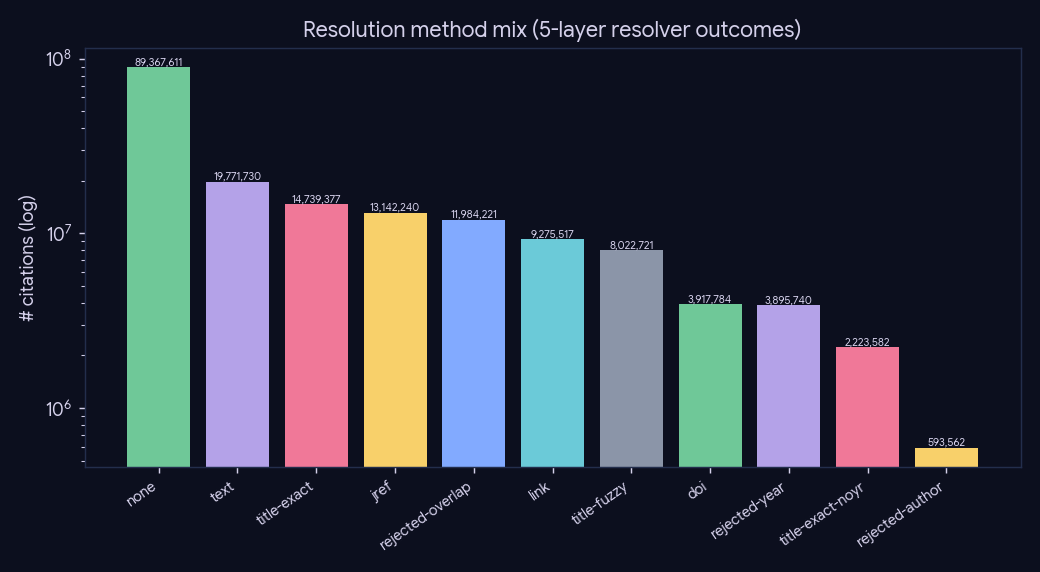
\includegraphics[width=0.85\textwidth]{../results/method_mix.png}\end{center}

\subsection*{By field and era}
Resolution rate varies by field (HTML/LaTeX availability + citation style) and rises over time as
ar5iv HTML coverage improves.

\begin{center}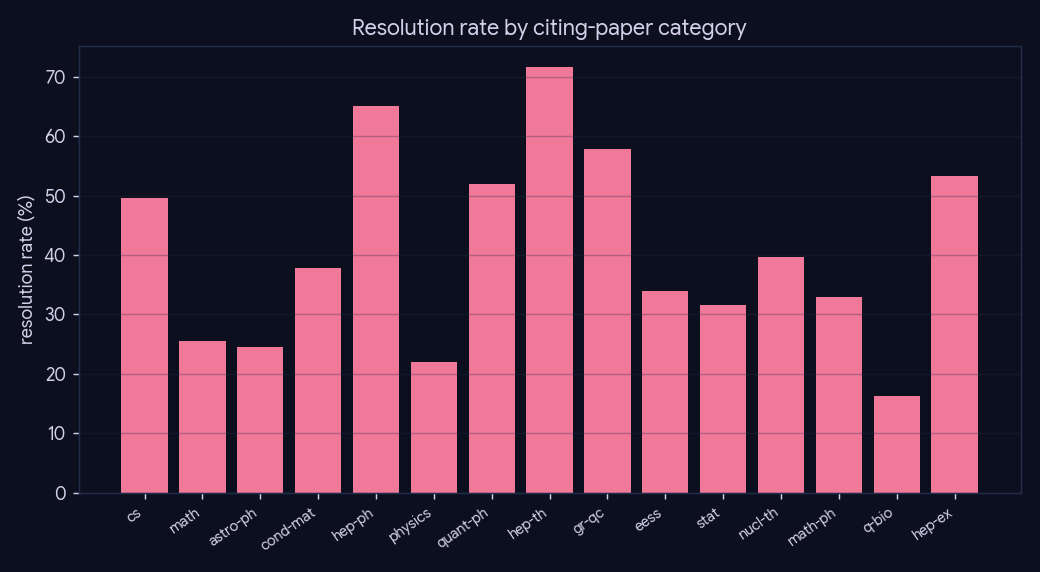
\includegraphics[width=0.78\textwidth]{../results/by_category.png}\end{center}
\begin{center}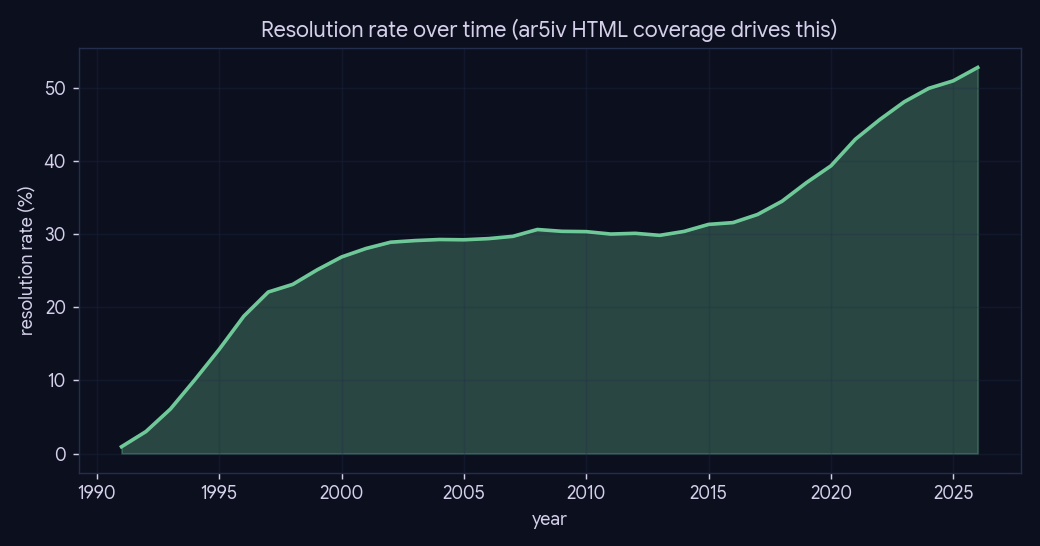
\includegraphics[width=0.78\textwidth]{../results/by_year.png}\end{center}

\section*{Conclusion}
The cheapest-first resolver resolves \textbf{40\,\%} of all citation occurrences corpus-wide, the
high-precision exact methods doing the bulk and the fuzzy layer adding a bounded $\sim$11\,\% tail
--- recall without leaning on the riskiest matcher. The remaining $\sim$60\,\%
\texttt{none}/\texttt{rejected-*} is dominated by citations to non-arXiv venues with no arXiv id to
resolve to. \texttt{rejected-*} rows are kept deliberately so the fuzzy layer's precision/recall
trade-off is visible, not silently dropped.

\end{document}
